\documentclass[problem]{mcs}

\begin{pcomments}
  \pcomment{CP_build_MSTs}
  \pcomment{ARM 10/27/11}
  \pcomment{F11.cp9m}
  \pcomment{figure addded 10/20/15}
\end{pcomments}

\pkeywords{
 spanning_tree
 weighted_tree
 minimum_weight
 MST
}

%%%%%%%%%%%%%%%%%%%%%%%%%%%%%%%%%%%%%%%%%%%%%%%%%%%%%%%%%%%%%%%%%%%%%
% Problem starts here
%%%%%%%%%%%%%%%%%%%%%%%%%%%%%%%%%%%%%%%%%%%%%%%%%%%%%%%%%%%%%%%%%%%%%

\begin{problem}
Let $G$ be the $4 \times 4$ grid with vertical and horizontal edges
between neighboring vertices and edge weights as shown in
Figure~\ref{fig:4x4}.

In this problem you will practice some of the ways to build minimum
weight spanning trees.  For each part, list the edge weights in the
order in which the edges with those weights were chosen by the given
rules.

\iffalse
  Formally,
\[
\vertices{G} = [0,3]^2 \eqdef \set{(k,j) \suchthat 0 \leq k,j \leq 3}.
\]
Letting $h_{i,j}$ be the horizontal edge $\edge{(i,j)}{(i+1,j)}$ and
$v_{j,i}$ be the vertical edge $\edge{(j,i)}{(j,i+1)}$ for $i\in[0,2],
j \in [0,3]$, the weights of these edges are
\begin{align*}
w(h_{i,j}) & \eqdef  \frac{4i+j}{100},\\
w(v_{j,i}) & \eqdef 1+\frac{i+4j}{100}.
\end{align*}
\fi

%\begin{center}
\label{fig:4x4}
\begin{figure}[h]
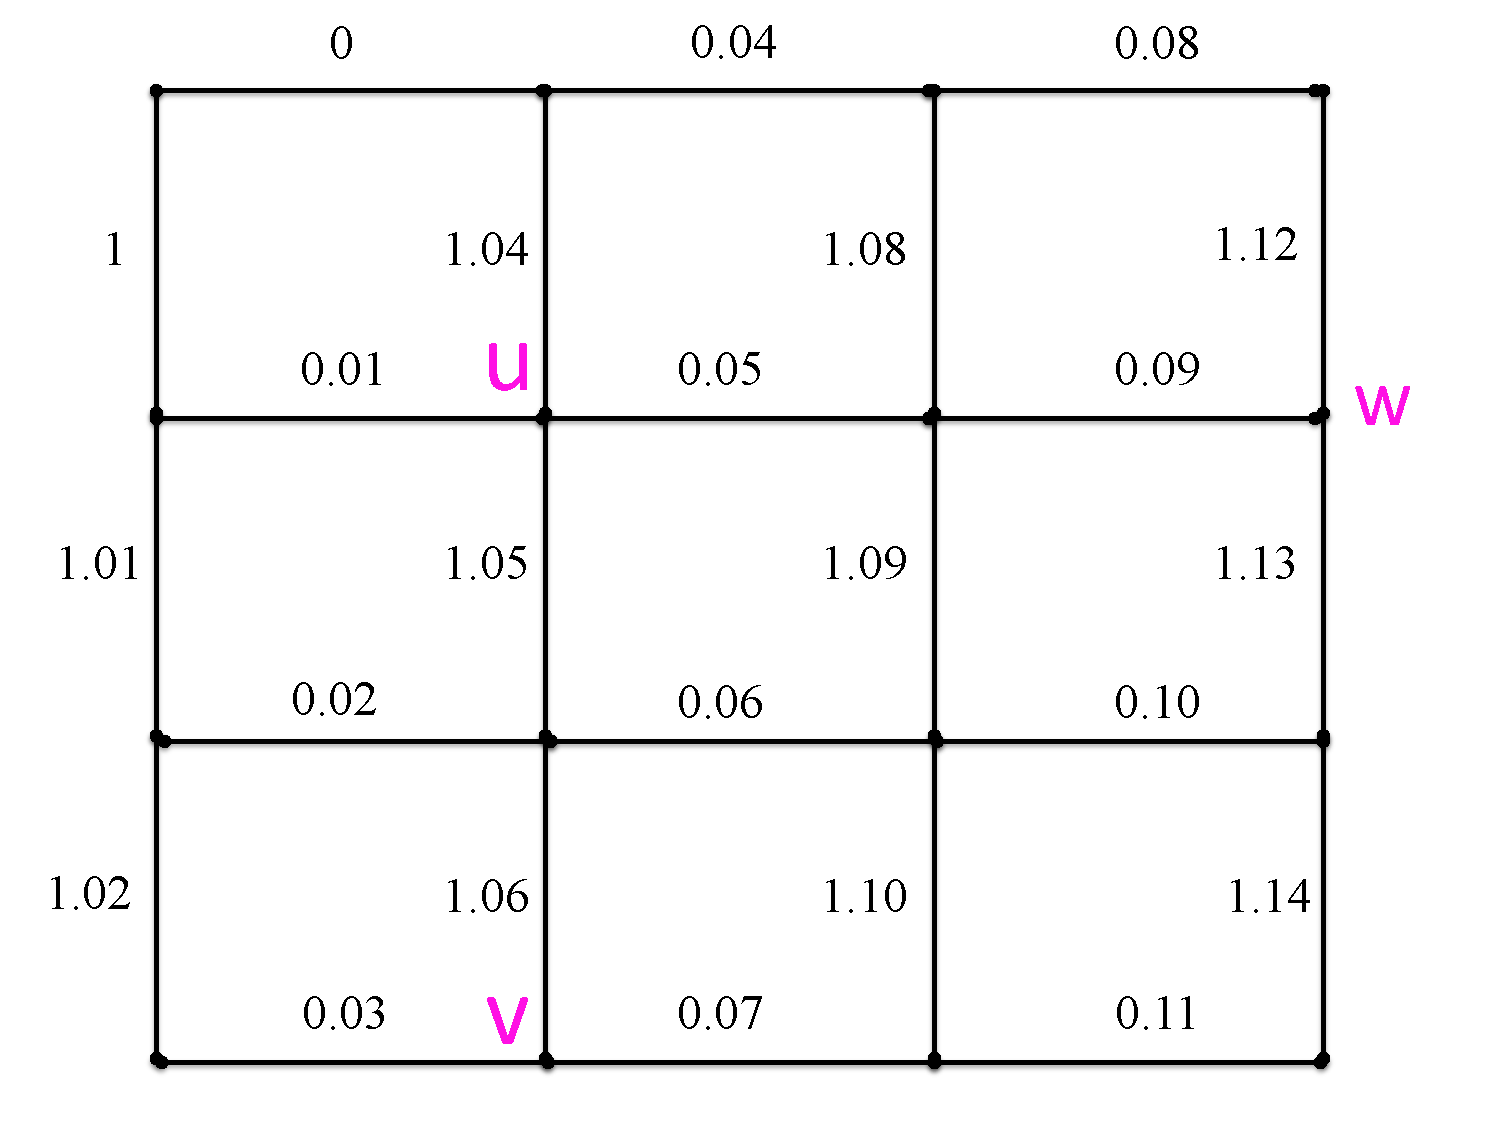
\includegraphics[height=4in]{4x4-array.pdf}
\caption{4x4 array graph}
%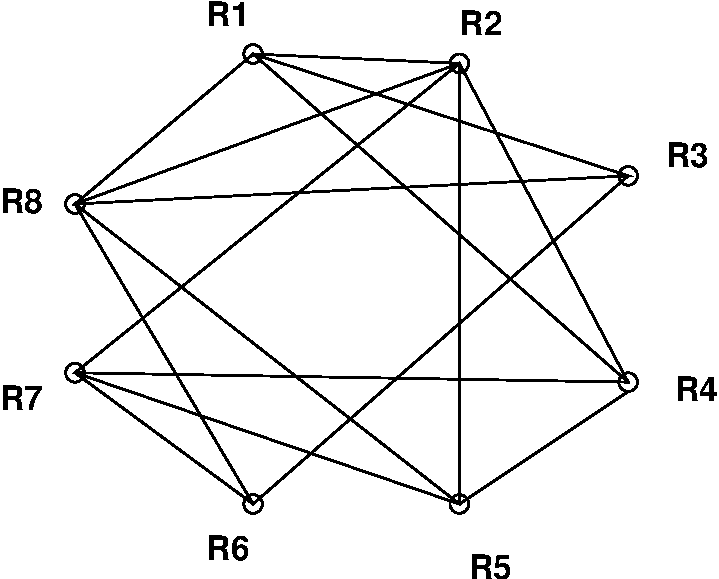
\includegraphics[height=5in]{ps3-schedule}
\end{figure}
%\end{center}

\bparts

\ppart Construct a minimum weight spanning tree (MST) for $G$ by
initially selecting the minimum weight edge, and then successively
selecting the minimum weight edge that does not create a cycle with
the previously selected edges.  Stop when the selected edges form a
spanning tree of $G$.  (This is Kruskal's MST algorithm.)

\inhandout{For any step in Kruskal's procedure, describe a black-white
  coloring of the graph components so that the edge Kruskal chooses is
  the minimum weight ``gray edge'' according to
  Lemma~\bref{lem:edgeextends}.}

\begin{staffnotes}
This problem can become a tedious time-sink.  If it takes more than 20
minutes, abort it, and explain the black-white coloring rules that
justify the first two parts.
\end{staffnotes}

\begin{solution}

The edge weights are listed in the order in which the edges with those
weight were chosen by the given algorithm.
\begin{staffnotes}
\TBA{CHECK THE ANSWER}

\end{staffnotes}
\[
0,.01,.02,.03,.04,.05,.06,.07,.08,.09,.010,.011,1,1.01,1.02
\]

\inhandout{From the text: An edge does not create a cycle iff it connects
different components.  The edge chosen by Kruskal's algorithm will be
the minimum weight gray edge when the components it connects are
assigned different colors.}

\end{solution}

\ppart Grow an MST for $G$ by starting with the tree consisting of the
single vertex incident to the edges with weights 0.01 and 0.05 and
successively adding the minimum weight edge with exactly one endpoint
in the tree.  Stop when the tree spans $G$.  (This is Prim's MST
algorithm.)

\inhandout{For any step in Prim's procedure, describe a black-white
  coloring of the graph components so that the edge Prim chooses is
  the minimum weight ``gray edge'' according to
  Lemma~\bref{lem:edgeextends}.}

\begin{solution}

\begin{staffnotes}

%$h_{0,2}h_{1,2}h_{2,2}v_{0,1}h_{0,1}h_{1,1}h_{2,1}v_{0,0}h_{0,0}h_{1,0}h_{2,0}v_{0,2}h_{0,3}h_{1,3}h_{2,3}$

\TBA{NEEDS CHECKING:}

\[
.01, .05, .09, 1, 0, .04, .08, .09, 1, .02, .06, .10, 1.02, .03, .07, .011
\]

\end{staffnotes}


\inhandout{From the text: This is the algorithm that comes from coloring the
growing tree white and all the vertices not in the tree black.  Then
the gray edges are the ones with exactly one endpoint in the tree.
}
\end{solution}


\ppart Grow an MST for $G$ by regarding the vertices at
\begin{itemize}
\item the upper left corner,
\item the upper right corner, and
\item bottom, one in from the left,
\end{itemize}
as three 1-vertex trees.  Successively add, for each tree in
parallel, the minimum weight edge among the edges with one endpoint in
the tree.  Continue as long as there is no edge between two trees,
then go back to applying the general gray-edge method until the
parallel trees merge to form a spanning tree of $G$.  (This is 6.042's
parallel MST algorithm.)

\begin{solution}

\TBA{UPDATE EDGE NAMES}

Done in parallel:

T1@(0,0): $h_{0,0}h_{1,0}h_{2,0}v_{0,0}h_{0,1}h_{1,1}h_{2,1}$

T2@(0,3): $h_{0,3}h_{2,3}v_{0,2}h_{0,2}h_{1,2}h_{2,2}v_{0,1}$ (merges with T1)

T3@(2,3): $h_{1,3}$ (merges with T2)
\end{solution}

\ppart Verify that you got the same MST each time.

\begin{solution}
They are the same---if no mistake was made.
Problem~\bref{PS_unique_MST} explains why there is a unique MST for
any finite connected weighted graph where no two edges have the same
weight.
\end{solution}

\eparts

\end{problem}

%%%%%%%%%%%%%%%%%%%%%%%%%%%%%%%%%%%%%%%%%%%%%%%%%%%%%%%%%%%%%%%%%%%%%
% Problem ends here
%%%%%%%%%%%%%%%%%%%%%%%%%%%%%%%%%%%%%%%%%%%%%%%%%%%%%%%%%%%%%%%%%%%%%

\endinput
